\documentclass{beamer}
%\usetheme{Boadilla}

\title{Bayesian Optimization}
\author{Steven}
\usepackage[utf8]{inputenc}
\usepackage{algpseudocode}
\usepackage{algorithm}
\usepackage[T1]{fontenc}
\usepackage{textcomp}
\usepackage[english]{babel}
\usepackage{verbatim}
\usepackage{cite}
%\setlist[enumerate]{ label=\arabic*.}


% Hide page number when page is empty
\usepackage{multicol}
\usepackage{xcolor}
% Other font I sometimes use.
% \usepackage{cmbright}

% Math stuff
\usepackage{amsmath, amsfonts, mathtools, amsthm, amssymb}
% Fancy script capitals
\usepackage{mathrsfs}
% Bold math
\usepackage{bm}


% Operators
\DeclareMathOperator{\Bd}{Bd}
\DeclareMathOperator{\Int}{Int}
\DeclareMathOperator{\cif}{if\;}

\DeclareMathOperator{\Var}{Var}
\DeclareMathOperator{\SD}{SD}
\DeclareMathOperator{\Cov}{Cov}
\DeclareMathOperator{\Cor}{Cor}
\DeclareMathOperator{\Pois}{Pois}
\DeclareMathOperator{\Dir}{Dir}
\DeclareMathOperator{\Unif}{Unif}
\DeclareMathOperator{\Gam}{Gamma}
\DeclareMathOperator{\Binom}{Binom}
\DeclareMathOperator{\Expo}{Expo}
\DeclareMathOperator{\dBeta}{dBeta}
\DeclareMathOperator{\tBeta}{tBeta}
\DeclareMathOperator{\Ber}{Ber}
\DeclareMathOperator{\IG}{IG}
\DeclareMathOperator{\Pb}{Pr}
\DeclareMathOperator*{\argmax}{arg\,max}
\DeclareMathOperator*{\argmin}{arg\,min}
\newcommand\deq{\stackrel{\mathclap{\tiny\mbox{d}}}{=}}
\def\bsy{\boldsymbol}



\begin{document}
\begin{frame}
    \titlepage
\end{frame}

\begin{frame}
    \frametitle{Motivation}
    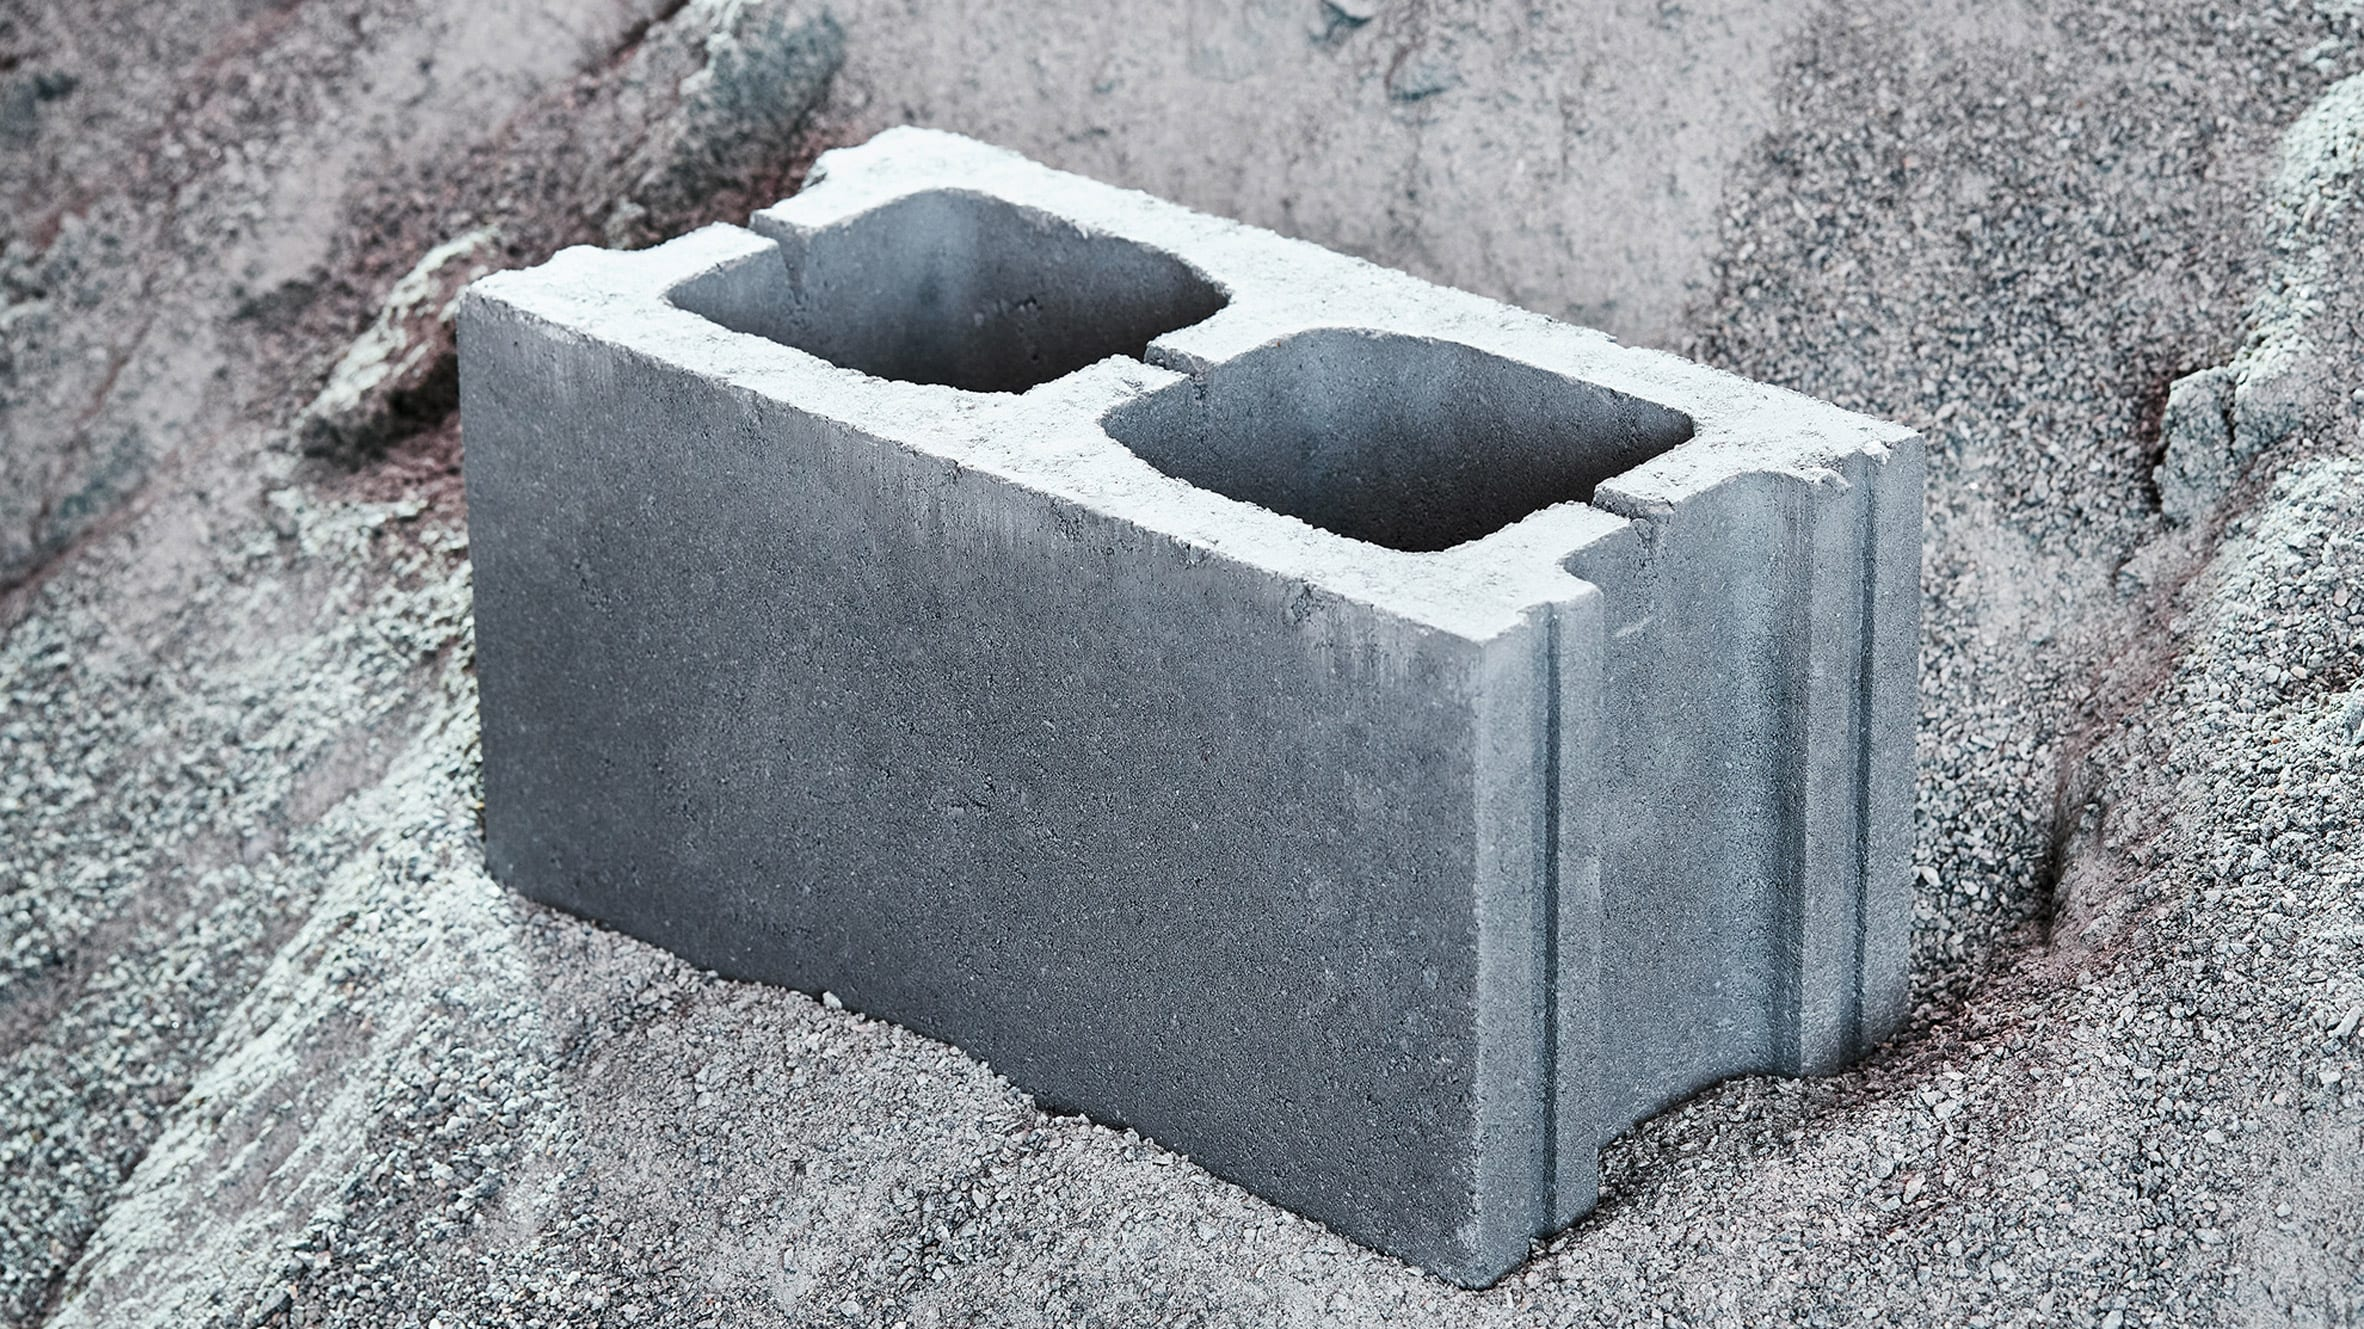
\includegraphics[width=0.49\textwidth]{fig/carbon-neutral-concrete-feature_dezeen_2364_col_1.jpg}
    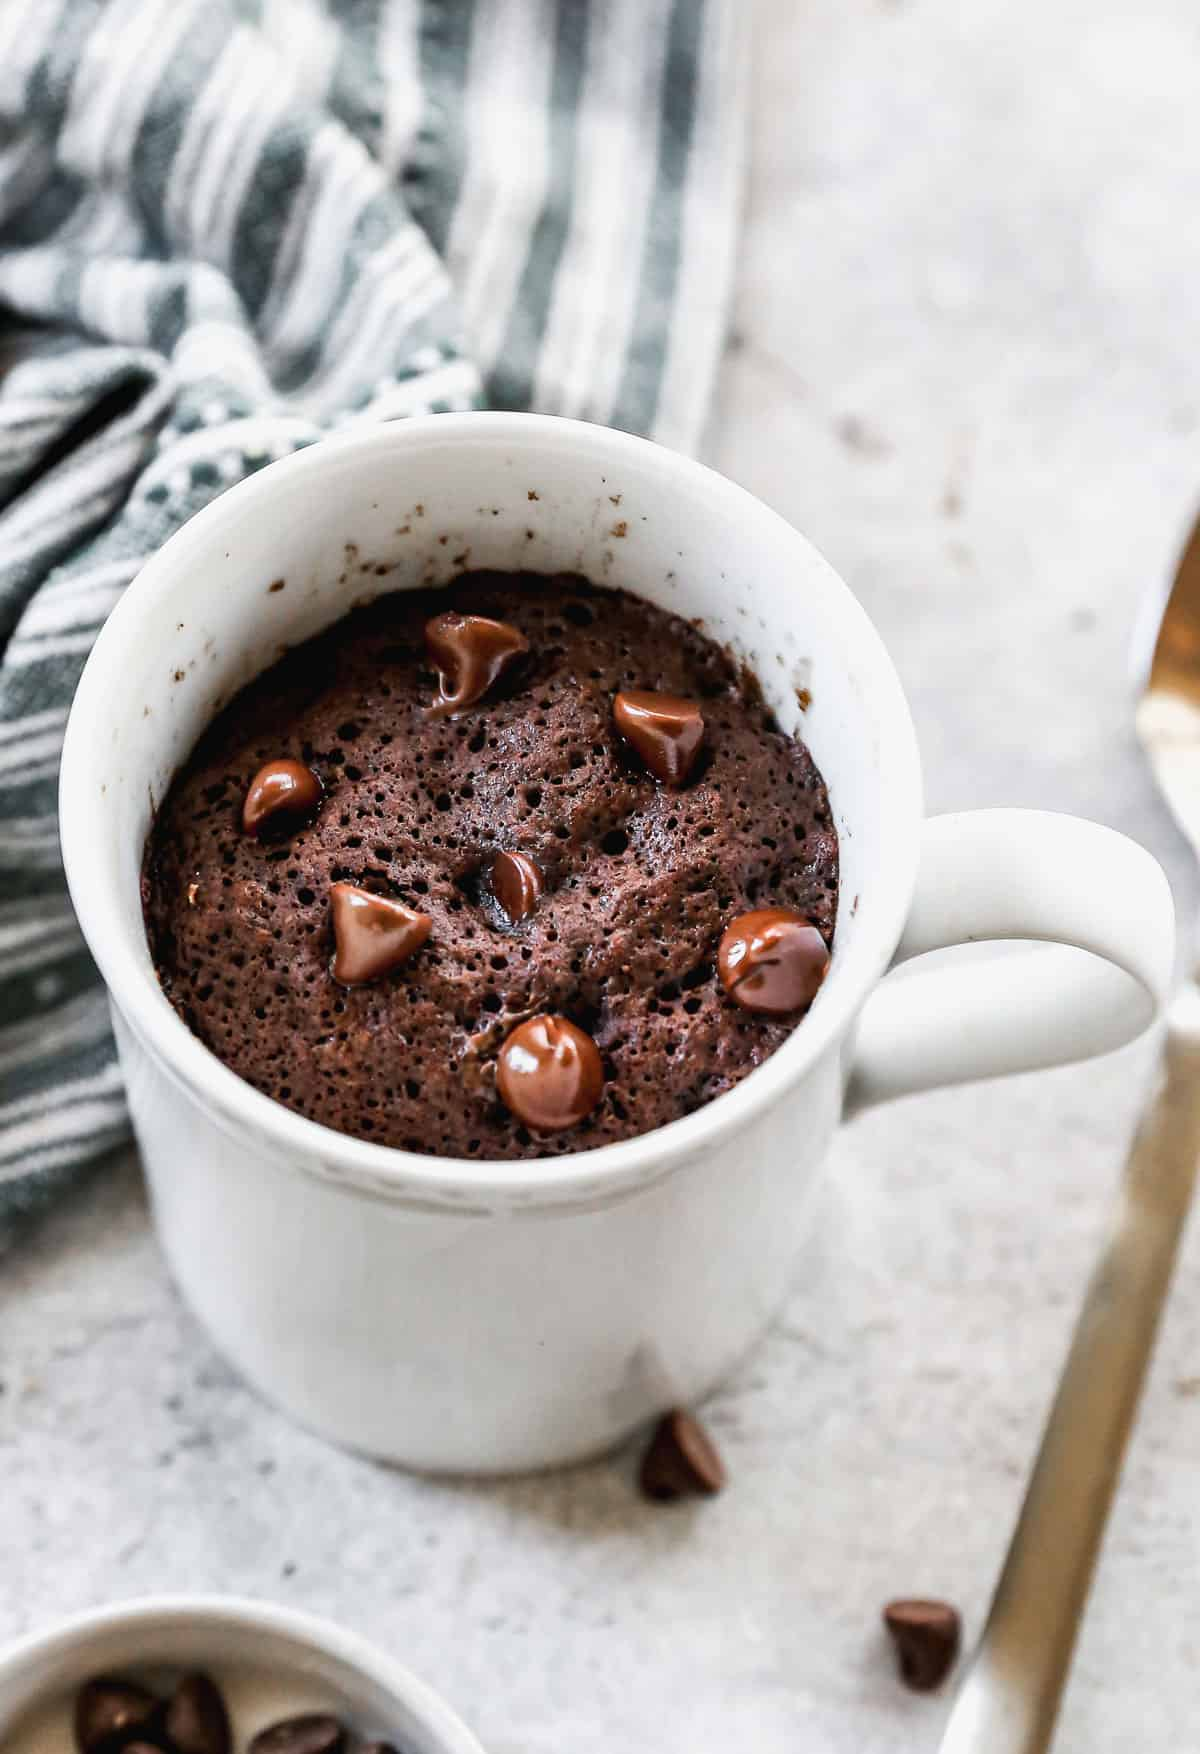
\includegraphics[width=0.49\textwidth]{fig/Chocolate-Mug-Cake-1.jpg}
\end{frame}

\begin{frame}
    \frametitle{Big Idea}
    For some unknown continuous function $f$ from a compact set $\mathcal{X} \subseteq \mathbb{R}^{K}$ to $\mathbb{R}$, we want to find
    \begin{equation*}
        \argmin_{\mathbf{x} \in \mathcal{X}} f(\mathbf{x})
    \end{equation*}
    in as few noisy samples as possible.
\end{frame}

\begin{frame}
    \begin{centering}
        https://www.cs.middlebury.edu/\textasciitilde sjinxuan/output.gif
    \end{centering}
\end{frame}

\begin{frame}
    \frametitle{Connections to Other Class}
    \begin{itemize}
        \item Stochastic Processes: Working with infinite sets of random variables.
        \item Real Analysis: $\epsilon-\delta$ proofs.
        \item Calculus: Gradient based optimization.
        \item Bayesian Stats: Priors, posteriors, credible intervals, etc.
    \end{itemize}
\end{frame}

\begin{frame}
    \frametitle{Learning}

    \begin{itemize}
        \item
            How to write and test code that is both maintainable and efficient.
        \item
            Measure-theoretic understanding of probability.
        \item
            Infinite-dimensional linear algebra.
    \end{itemize}
\end{frame}

\begin{frame}
    \frametitle{Progress}
    Done some writing, still need to do real experiments.
\end{frame}

\end{document}
